\chapter{Implementation}


The various stages in the implementation of the proposed system are as\\ follows:\\

\section{User Interface}
First the user selects the database of choice. Now the user can input the natural language query in the user interface. The user interface is meant so that the user can aid the system in query translation. The user plays an integral role in node mapping, discussed in section \ref{mapping}.
\section{Schema Graph}
The database schema taken from the underlying database is represented as follows:
\begin{itemize}
\item There are two types of nodes. 
\subitem{Relation Nodes(RN) : to represent the relations} 
\subitem{Attributes Nodes(AN) : to represent the attributes of the relations}
\item Similarly, there are two types of edges. 
\subitem{Relation Edges : to represent the foreign key-primary key relationship.} 
\subitem{Attributes Edges : to represent the attributes of the relations. For every RN there is a edge from it to all the AN which represents the attribute of the corresponding relation.}
\end{itemize}

\begin{algorithm}[Q]
\SetAlgoLined




\SetKwInOut{Input}{input}\SetKwInOut{Output}{output}
\Input{A Database \textbf{db} }
\Output{Schema Graph \textbf{S(V,E)} representing \textbf{db}}
\BlankLine




\textbf{dbSchema} $\leftarrow$ \emph{extract schema from } \textbf{db}

\textbf{keyRelations} $\leftarrow$ \emph{ extract primary key - foreign key relations from } \textbf{dbSchema} 

\textbf{tables} $\leftarrow$ \emph{ extract table names from } \textbf{dbSchema} \;

\ForEach{ \emph{tableName} \in \textbf{tables}}{
    
    \textbf{\emph{columns}}\emph{[tableName]} $\leftarrow$  \emph{extract all attributes of tableName from } \textbf{dbSchema}
 
}

\textbf{S(V,E)} $\leftarrow \phi$

\ForEach{ \emph{tableName} \in \textbf{tables}}{
    \textbf{S(V)}.add(makeRelationNode(tableName))
    
  

}


\ForEach{ \emph{(FK,PK)} \in \textbf{tables}}{
    \textbf{S(E)}.addDirectedEdge(FK, PK)
}

\ForEach{colName \in \textbf{columns}[tableName]}{
        \textbf{S(V)}.addAttributeNode(colName)
    }

\ForEach{ \emph{tableName} \in \textbf{tables}}{

    \ForEach{colName $\in$ \textbf{columns}[tableName]}{
        \textbf{S(E)}.addDirectedEdge(tableName, colName)\\
        \textbf{\emph{sampleData}}\emph{[columnName]} $\leftarrow$ \emph{extract \emph{t} samples from columnName of tableName using } \textbf{db}  
    }
     
}
\textbf{Return} \textbf{\emph{S(V,E)}}
 \caption{Schema Graph Generation}
\end{algorithm}

\newpage

\section{Parse tree}
The natural language input is parsed using Stanford Parser.\cite{ten} This parse tree is used to understand the structure of the input. This parse tree has the following different type of nodes,


The stanford parser gives a tree of words. For each of these words in the parse tree we create a corresponding node in our parse tree with the word as its value and the tree structure is maintained. 


\begin{figure}[htb]
\centering
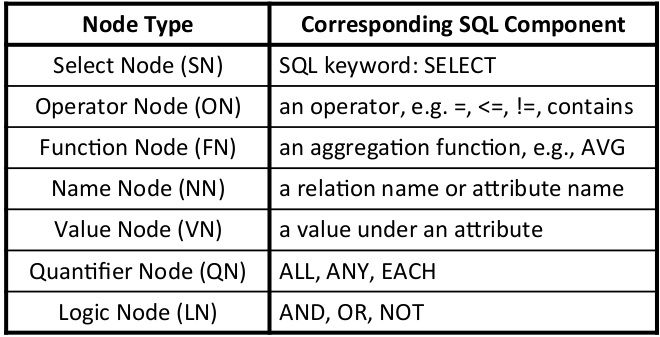
\includegraphics[scale=0.55]{nodes} % e.g. insert ./image for image.png in the working directory, adjust scale as necessary
\caption{Parse tree nodes}
\label{fig:aa} % insert suitable label, this is used to refer to a fig from within the text as shown above
\end{figure}


The figure \ref{fig:vv} is an example of a parse tree generated by the stanford parser,
\newpage


\begin{figure}[htb]
\centering
\includegraphics[scale=0.5]{pt} % e.g. insert ./image for image.png in the working directory, adjust scale as necessary
\caption{Parse tree for the NL query}
\label{fig:vv} % insert suitable label, this is used to refer to a fig from within the text as shown above
\end{figure}

\section{SQL Query Grammar }
The figure \ref{fig:grammara} shows is the grammar used to represent an SQL query in this project,

\begin{figure}[htb]
\centering
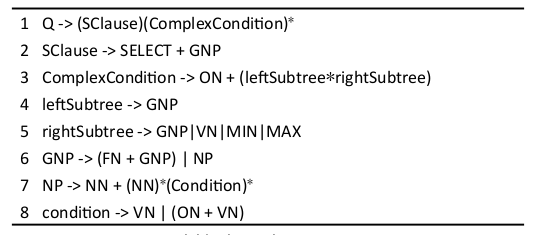
\includegraphics[scale=0.45]{./gram} % e.g. insert ./image for image.png in the working directory, adjust scale as necessary
\caption{Grammar for a SQL query}
\label{fig:grammara} % insert suitable label, this is used to refer to a fig from within the text as shown above
\cite{eleven}
\end{figure}

\newpage
In Figure \ref{fig:grammara},
+ represents a parent-child relationship.
* represents a sibling relationship.
One Query (Q) can must have one SClause and zero or more ComplexConditions.
A ComplexCondition must have one ON, with a leftSubtree and a rightSubtree.
An NP is: one NN (since an SQL query has to select at least one attribute), whose children are multiple NNs and Conditions. (All other selected attributes and conditions are stacked here to form a wide "NP" tree.)\cite{eleven}\\
All the valid parse trees should be in accordance to this grammar. So our aim is to rearrange the parse tree so that it follows the grammar.

\section{Node mapping}\label{mapping}
The identification of select node, operator
node, function node, quantifier node and logic node is independent of the database being queried.
Name nodes and value nodes correspond to
the meta-data and data, respectively, which entirely depend
on the database being queried.
When a parse tree node has multiple candidates for mapping it into particular type of node then our system returns multiple candidate mappings for the user to choose from. Also the user may also specify that some words are meaningless or unknown to him. Such nodes have to be removed from the tree.



\begin{algorithm}[H]
\SetAlgoLined




\SetKwInOut{Input}{input}\SetKwInOut{Output}{output}
\Input{A parse tree from stanford parser \textbf{PT} }
\Output{Mapped Parse Tree}
\BlankLine

\ForEach{ \emph{node} $\in$ \textbf{PT}}{\If{node.value $\in$ keywords}{ 
        node.type = node.value \\
        \emph{continue}
    }
    
    \textbf{choicesToMap} $\leftarrow$ \emph{calculateChoices(node.value)}\\
    
    \textbf{userChoice} $\leftarrow$ ask user to choose from a set of choices $\in$ \textbf{choicesToMap } ordered in decreasing value of relevance \\
    node.type = userChoice
    
    
}


\textbf{Return} \textbf{PT}


 \caption{Node Mapping}
\end{algorithm}

\begin{algorithm}[Y]
\SetAlgoLined




\SetKwInOut{Input}{input}\SetKwInOut{Output}{output}
\Input{A parse tree node \textbf{node}, \textbf{schema graph S}, \textbf{WordNet}  }
\Output{List of mapping choices}
\BlankLine

\textbf{choices} $\leftarrow$ ()\\
\ForEach{colName $\in$ \textbf{S.columns}}{
    \emph{score $\leftarrow$ \textbf{WordNet.similarity}(colName, \textbf{node.value})}
    \emph{\textbf{choices}.append((colName,score,NN))}
}

\ForEach{tableName \in \textbf{S.tables}}{
    score = $\leftarrow$ \textbf{WordNet.similarity}(tableName, \textbf{node.value})
    \textbf{choices}.append((tableName,score,NN))
}

\ForEach{colName \in \textbf{S.columns}}{
    \textbf{score} $\leftarrow$ \emph{1}\\
    \ForEach{\emph{data} $\in$ \textbf{S.sampleData}[columns]}{
        \textbf{score}*=\textbf{WordNet.similarity}(node.value,data)
        \textbf{choices}.append((colName,score,NV))
    }
    
}
\textbf{Return} \textbf{\emph{choices}}
 \caption{calculateChoices()}
\end{algorithm}

The node mapping is done with the help of user interaction. The user selects the node type from a list of possible types ordered in decreasing order of its score. Score of type for a particular node is calculated by finding out the similarity between them. The similarity measure used is from WordNet. 




\begin{figure}[htb]
\centering
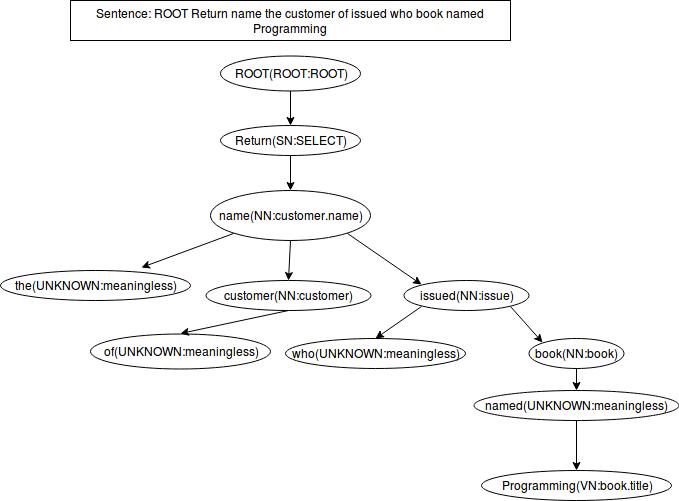
\includegraphics[scale=0.45]{./map} % e.g. insert ./image for image.png in the working directory, adjust scale as necessary
\caption{Parse after node mapping }
\label{fig:grammar} % insert suitable label, this is used to refer to a fig from within the text as shown above
\end{figure}




\begin{figure}[htb]
\centering
\includegraphics[scale=0.45]{./rem} % e.g. insert ./image for image.png in the working directory, adjust scale as necessary
\caption{Parse after removing meaningless nodes}
\label{fig:grammar} % insert suitable label, this is used to refer to a fig from within the text as shown above
\end{figure}







\section{Rearrangement of parse tree}
After all the nodes of the parse tree is mapped,the tree can be understood by the system. But linguistic parse tree generated from a parser may be incorrect as natural language sentences often have complex structures and also such parse trees may not be completely in adherence of the SQL query grammar. So the parse tree has to be rearranged to get a suitable tree.\\








\begin{algorithm}[J]
\SetAlgoLined
\SetKwInOut{Input}{input}\SetKwInOut{Output}{output}


\Input{A parse tree \textbf{parseTree}  }
\Output{A list of relevant parse trees}


\BlankLine

\textbf{results} $\leftarrow$ \phi\\
\textbf{PriorityQ} $\leftarrow$ \phi\\
PriorityQ.insert(\textbf{parseTree})\\
\While{PriorityQ $\ne$ \phi}{
    Ptree = PriorityQ.remove()\\
    treeList = adjust(Ptree)\\
    \ForEach{tree $\in$ \emph{treeList}}{
        \If{tree.edit \textless t }{
            tree.edit += 1\\
            \If{evaluateScore(tree) $\ge$ evaluateScore(Ptree)}{
                PriorityQ.insert(tree')\\
                \If{tree is valid}{
                    \textbf{results}.append(tree)
                }
            }
        }
    }
}
\textbf{Return} \textbf{\emph{results}}

 \caption{Tree Rearrangement}
\end{algorithm}







\begin{algorithm}[K]
\SetAlgoLined
\SetKwInOut{Input}{input}\SetKwInOut{Output}{output}


\Input{A parse tree \textbf{parseTree}  }
\Output{A list parse trees }


\BlankLine

\textbf{adjustedTrees} $\leftarrow$ \phi\\

\ForEach{\emph{node} $\in$ \textbf{\emph{parseTree}}}{
    \ForEach{child in \emph{node}}{
        \textbf{\emph{adjustedTrees}}.add(swap \emph{node} and child)\\
        \textbf{\emph{adjustedTrees}}.add(make \emph{node} its sibling)\\
        \textbf{\emph{adjustedTrees}}.add(make siblings the child of \emph{node})\\
        \textbf{\emph{adjustedTrees}}.add(swap \emph{node's} children)\\
    }
    
}

\textbf{Return} \textbf{\emph{adjustedTrees}}

 \caption{adjust()}
\end{algorithm}





\begin{figure}[htb]
\centering
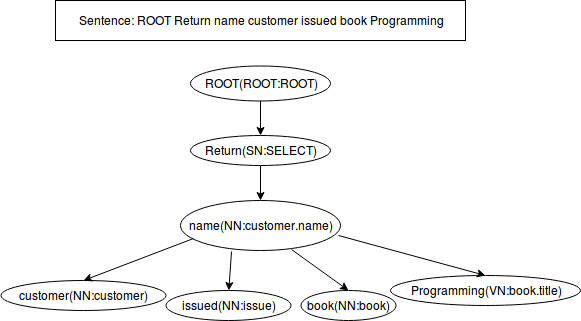
\includegraphics[scale=0.45]{./tran} % e.g. insert ./image for image.png in the working directory, adjust scale as necessary
\caption{Best rearranged parse tree for the query}
\label{fig:grammar} % insert suitable label, this is used to refer to a fig from within the text as shown above
\end{figure}

The basic idea is to move sub-trees to edit the parse tree until it is syntactically correct according to the grammar defined.Each time, we use the move function we  generate all the possible parse trees in one
sub-tree move operation. The number of parse trees grows exponentially with the number of edits. To fasten the process,
 each new generated parse tree is evaluated and
 bad parse trees directly filtered out. We also set a parameter as the
maximum number of edits approved. Our system
records all the valid parse trees appeared in the reformulation process and returns the top k of them so that the user can choose from them.\\
Now to rate each of the generated parse trees in the method above we set the score of the parse tree as the negative of the number of invalid nodes it has. A node is said to be invalid if that node does not follow the grammar defined for SQL queries.



\section{SQL query generation}
Last step in our process is to generate SQL query from query tree. Since the parse tree now adheres to the SQL grammar the we have defined the translation is done directly according to it. The schema element mapped by the node which has similarity between label and schema element name, under the SELECT node is added
to the SELECT clause. Each value node is transformed to a selection condition and added to the WHERE clause. Finally, a foreign key-primary key
join path is generated, according to the schema graph, to
connect each nodes in the select clause and its neighbors. Such an foreign key-primary key join path is translated into a series of foreign key-primary key join conditions and all the schema elements in the foreign key-primary key join path are added to the FROM clause.\cite{eleven}




